\documentclass[a4paper]{article}

\usepackage{fontspec}
\usepackage{tikz}
\usetikzlibrary{calc}
\usepackage[dvipsnames]{xcolor}

\definecolor{mygray}{gray}{0.6}
\setmainfont{SFUIDisplay-Light.ttf}

\title{\vspace{-4cm}\hspace*{-16.0cm}\textcolor{mygray}{\large{Prototyping Papers}} \\ 
       \hspace*{-15.2cm}\huge{Dotted paper.}}
\date{}

\begin{document}
\maketitle

\begin{tikzpicture}[overlay, remember picture]
\node[anchor=north west, 
      xshift=17cm,
      yshift=-1.0cm] 
     at (current page.north west) 
     {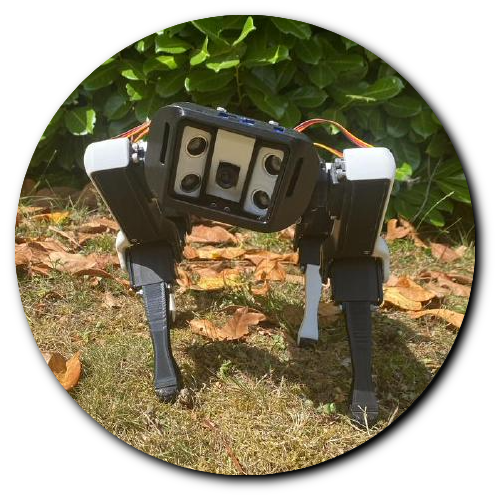
\includegraphics[width=3cm]{shadowed_example_pfp.png}}; 
\end{tikzpicture}

\begin{tikzpicture}[overlay]
    \foreach \x in {-8,...,30}
    \foreach \y in {-44,...,2}
    { \fill[gray!75] (0.5*\x,0.5*\y) circle (0.03cm); }       
\end{tikzpicture}

\setlength{\footskip}{100pt}

\renewcommand{\thepage}{\scriptsize{Supporting open source. Visit \url{https://github.com/vertueux/prototyping-papers} for the copy and use of this paper.}}

\end{document}